\chapter*{Chiloe : journée à Puñihuil\markboth{Chiloe : journée à Puñihuil}{}}
\section*{18 février 2015}
Enfin une journée qui s´annonce sous le soleil ! \newline
 \newline
\centerline{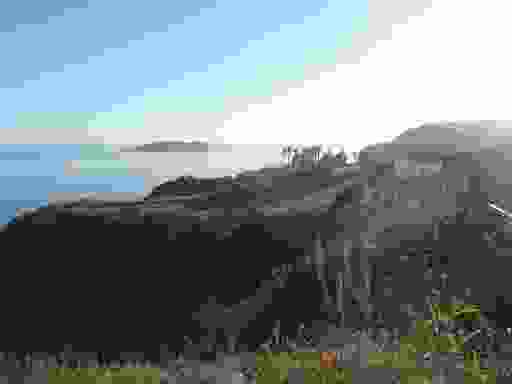
\includegraphics[width=\mywidth]{../wp-content/uploads/2015/02/P2122067.jpg} } 
 \newline
 30km de belle route le long de la côte pour aller à la Pinguineria de Puñihuil. \newline
 \newline
\centerline{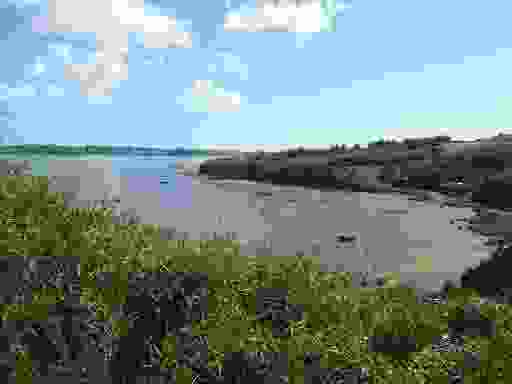
\includegraphics[width=\mywidth]{../wp-content/uploads/2015/02/P2122070.jpg} } 
 \newline
\centerline{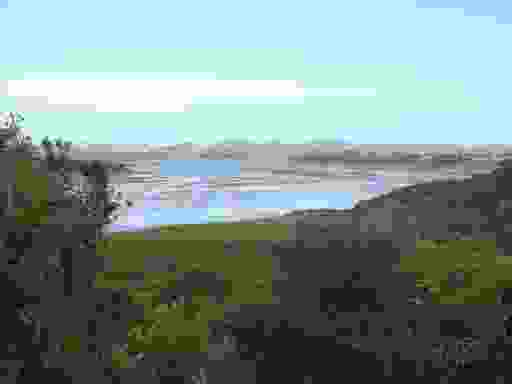
\includegraphics[width=\mywidth]{../wp-content/uploads/2015/02/P2122072.jpg} } 
 \newline
\centerline{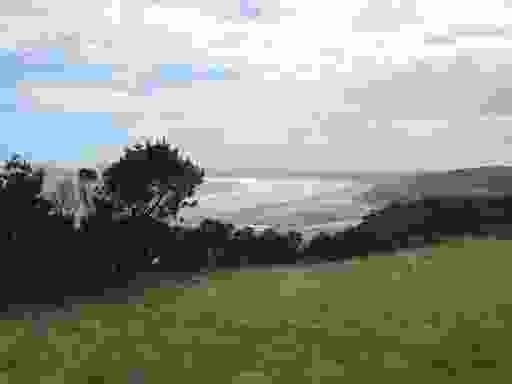
\includegraphics[width=\mywidth]{../wp-content/uploads/2015/02/P2122073.jpg} } 
 \newline
\centerline{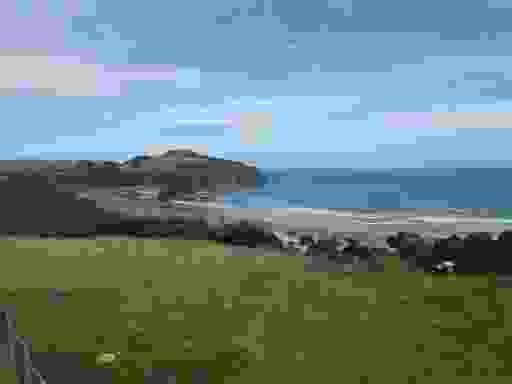
\includegraphics[width=\mywidth]{../wp-content/uploads/2015/02/P2122074.jpg} } 
 \newline
\centerline{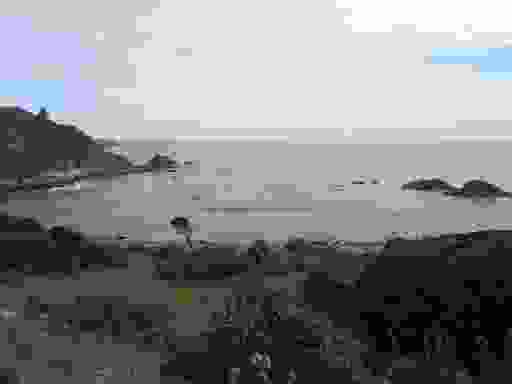
\includegraphics[width=\mywidth]{../wp-content/uploads/2015/02/P2122075.jpg} } 
 Rencontre avec Carlo, un cycliste italien \newline
 \newline
\centerline{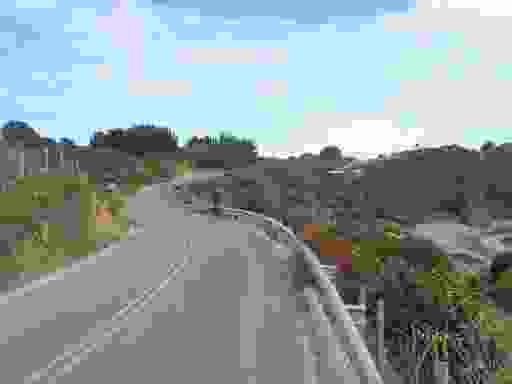
\includegraphics[width=\mywidth]{../wp-content/uploads/2015/02/P2122077.jpg} } 
 Tour en bateau depuis la plage \newline
 \newline
\centerline{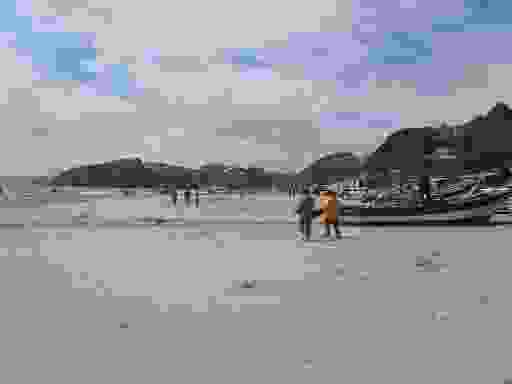
\includegraphics[width=\mywidth]{../wp-content/uploads/2015/02/P2122079.jpg} } 
 \newline
\centerline{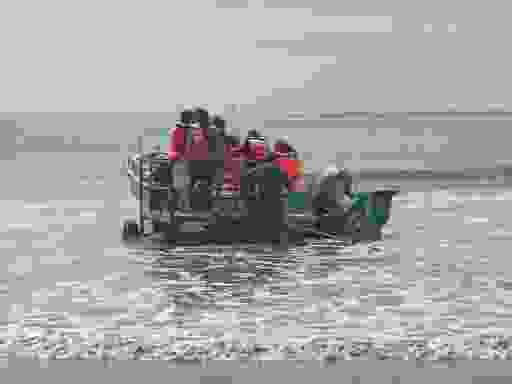
\includegraphics[width=\mywidth]{../wp-content/uploads/2015/02/P2122080.jpg} } 
 Il y a 2 espèces différentes de pingouins sur l´ìle. \newline
\centerline{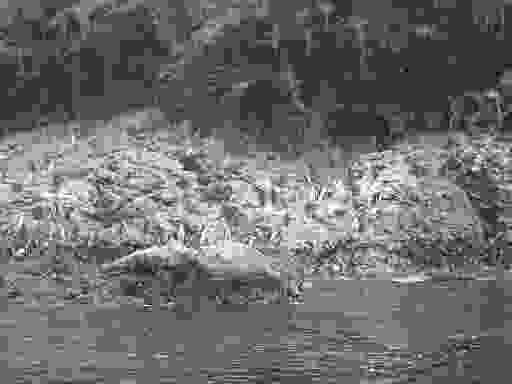
\includegraphics[width=\mywidth]{../wp-content/uploads/2015/02/P2122084.jpg} } 
 \newline
\centerline{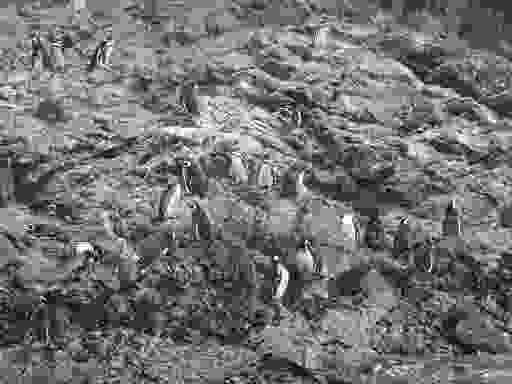
\includegraphics[width=\mywidth]{../wp-content/uploads/2015/02/P2122087.jpg} } 
 \newline
\centerline{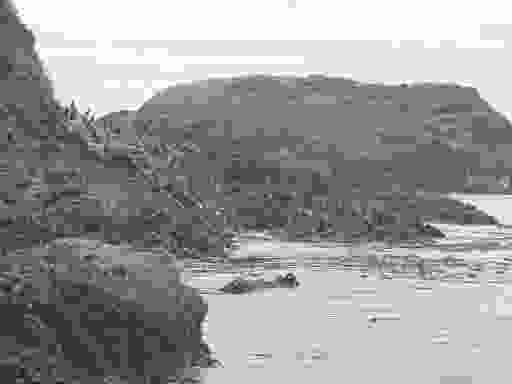
\includegraphics[width=\mywidth]{../wp-content/uploads/2015/02/P2122088.jpg} } 
 Des pelicans \newline
\centerline{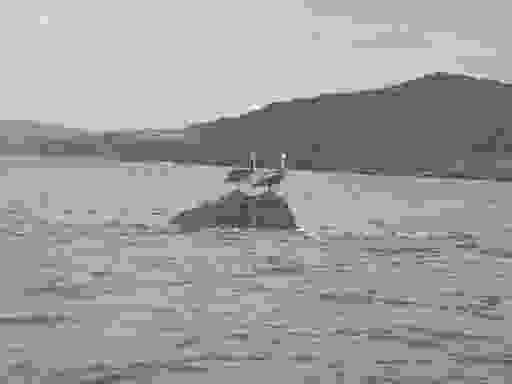
\includegraphics[width=\mywidth]{../wp-content/uploads/2015/02/P2122094.jpg} } 
 Je reprend la route avec Carlo sur un chemin en gravier qui enchaîne montées et descentes raides. \newline
 Trop difficile pour mon vélo : le filetage qui fixe les pignons au moyeu est mort et je ne peux plus avancer car je pédale dans le vide. \newline
 \newline
\centerline{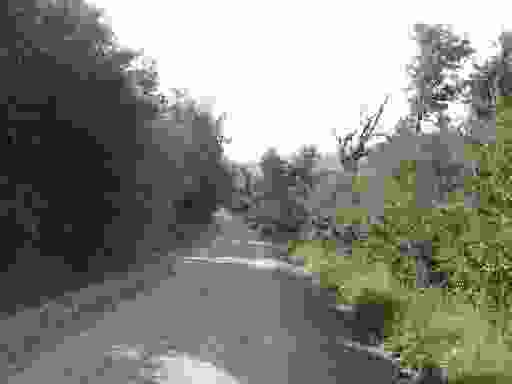
\includegraphics[width=\mywidth]{../wp-content/uploads/2015/02/P2122095.jpg} } 
 Demi tour pour rejoindre la route à pied : par chance un pick up s'arrête et accepte de me déposer à Ancud. \newline
 Changement du moyeu dans un magasin de vélo, le technicien est efficace il a démonté, remonté tous les rayons de la roue arrière et dévoilé la roue en à peine 1h et demie. \newline
 Du coup je retourne au même camping que la veille et je recroise Javier et Jonathan, 2 voyageurs à vélo que j´avais déjà rencontrés. \newline
 \newline
\centerline{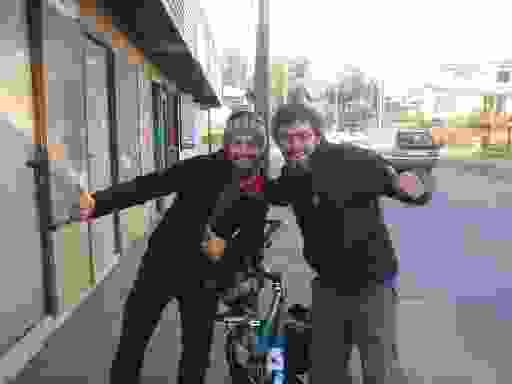
\includegraphics[width=\mywidth]{../wp-content/uploads/2015/02/P2132096.jpg} } 
 \newline

\newpage
 
